\documentclass[12pt,a4paperpaper,]{article}

\usepackage{lmodern}
\usepackage{amssymb,amsmath}

% use upquote if available, for straight quotes in verbatim environments
\IfFileExists{upquote.sty}{\usepackage{upquote}}{}
% use microtype if available
\IfFileExists{microtype.sty}{%
\usepackage{microtype}
\UseMicrotypeSet[protrusion]{basicmath} % disable protrusion for tt fonts
}{}

\usepackage{geometry}
\geometry{
    top=1in,
    bottom=1in,
    left=1in,
    right=1in,
    headheight=3ex,
    headsep=3ex
}
\usepackage{sidecap}
\usepackage{subfigure}

\usepackage[unicode=true]{hyperref}
\hypersetup{
            pdftitle={Attention in value-based choice as optimal sequential sampling},
            pdfborder={0 0 0},
            breaklinks=true}
\urlstyle{same}  % don't use monospace font for urls

% \usepackage[natbibapa]{apacite}
\usepackage{natbib}
% \bibliographystyle{apacite}
\bibliographystyle{apalike}
% \citationstyle{apacite}
% \bibpunct{[}{]}{,}{n}{}{;}


\usepackage{graphicx,grffile}
\makeatletter
\def\maxwidth{\ifdim\Gin@nat@width>\linewidth\linewidth\else\Gin@nat@width\fi}
\def\maxheight{\ifdim\Gin@nat@height>\textheight\textheight\else\Gin@nat@height\fi}
\makeatother
% Scale images if necessary, so that they will not overflow the page
% margins by default, and it is still possible to overwrite the defaults
% using explicit options in \includegraphics[width, height, ...]{}
\setkeys{Gin}{width=\maxwidth,height=\maxheight,keepaspectratio}
\IfFileExists{parskip.sty}{%
\usepackage{parskip}
}{% else
\setlength{\parindent}{0pt}
\setlength{\parskip}{6pt plus 2pt minus 1pt}
}
\setlength{\emergencystretch}{3em}  % prevent overfull lines
\providecommand{\tightlist}{%
  \setlength{\itemsep}{0pt}\setlength{\parskip}{0pt}}
\setcounter{secnumdepth}{0}

% % Redefines (sub)paragraphs to behave more like sections
% \ifx\paragraph\undefined\else
% \let\oldparagraph\paragraph
% \renewcommand{\paragraph}[1]{\oldparagraph{#1}\mbox{}}
% \fi
% \ifx\subparagraph\undefined\else
% \let\oldsubparagraph\subparagraph
% \renewcommand{\subparagraph}[1]{\oldsubparagraph{#1}\mbox{}}
% \fi

% set default figure placement to htbp
\makeatletter
\def\fps@figure{htbp}
\makeatother


\usepackage{titlesec}

% % \titleformat*{\section}{\LARGE\bfseries\sffamily}
% % \titleformat*{\subsection}{\Large\bfseries\sffamily}
% % \titleformat*{\subsubsection}{\large\series}
% % \titleformat*{\paragraph}{\large\bfseries\sffamily}
% % \titleformat*{\subparagraph}{\large\bfseries\sffamily}

\titlespacing*{\section}{0pt}{3ex}{1ex}
\titlespacing*{\subsection}{0pt}{2ex}{0.5ex}
\titlespacing*{\subsubsection}{0pt}{1.5ex}{0.3ex}
\titlespacing*{\paragraph}{0pt}{1ex}{3ex}

%% Headers and footers:
%%
%% Center footer: page number
%% Right header:  nothing
%% Left header:   nothing
% \usepackage{lastpage}
% \newpagestyle{fancy}{
%   \setfoot{}{\thepage \ of \pageref*{LastPage}}{}
%   \sethead
%     { Attention in value-based choice as optimal sequential sampling }
%     {}
%     { Callaway }
%   \headrule
%   \setheadrule{0.3pt}
% }
% \pagestyle{fancy}  

\title{\vspace{-2em}Attention in value-based choice as optimal sequential sampling}
\author{Frederick Callaway \& Thomas L. Griffiths}

\date{\vspace{-1em}}

\begin{document}
\maketitle


\newcommand{\A}{\mathcal{A}}
\newcommand{\B}{\mathcal{B}}
\renewcommand{\S}{\mathcal{S}}
\newcommand{\D}{\mathcal{D}}
\newcommand{\R}{\mathbb{R}}
\newcommand{\Z}{\mathbb{Z}}
\newcommand{\expect}[2][]{\mathbb{E}_{#1} \left[ #2 \right]}
\newcommand{\nop}{\texttt{NOOP}}
\newcommand{\Normal}{\mathrm{Normal}}
\renewcommand{\vec}[1]{\mathbf{#1}}

Consider a diner at a new restaurant, perusing the menu and trying to decide what she wants to have for dinner. Under the standard model of economic decision making \citep{Kahneman1979,Rangel2008}, she would assign each item a value and then choose the one with maximal value. While her preferences might change day to day (leading to inconsistent choices), she always chooses the item that she likes best at the moment. Unfortunately, this idealization does not well capture the experience many of us have. Instead, we undergo a difficult and sometimes lengthy process of weighing the options, initially being drawn to one entr\'ee before identifying a competitor, oscillating between them, failing to notice a desirable choice, and feeling pangs of regret at the sight of our companion's meal.

A great deal of work in psychology and neuroscience has attempted to better capture the process through which people make decisions. One key insight is that decision-making is a sequential process. This insight is formalized in the drift-diffusion model \citep{Ratcliff1978,Milosavljevic2010}, where the oscillation between mushroom risotto and pesto gnocchi is captured by the perturbations of a random walk. However such models fail to capture the important role that attention plays in the decision making process \citep{Orquin2013}. One primary empirical effect is that people are more likely to choose items that they look at more. This effect is captured by the attentional drift diffusion model (aDDM), which biases the drift rate in favor of the fixated item \citep{Krajbich2010}. In addition to explaining this basic effect of attention on choice, the aDDM predicts subtler patterns. For example, last fixations are predicted to be shorter than first fixations, because the fixation is cut off when the decision variable crosses a barrier.

% eye-mind assumption (see Orquin review)

Despite these successes, several important questions have not been addressed by previous work. The vanilla drift-diffusion model has been shown to be equivalent to a sequential probability ratio test \citep{Bogacz2006,Bitzer2014}, providing a rational explanation for why people might use a DDM-like decision mechanism. However, there is no such rational justification for why people would bias their choices with their attention. Indeed, it is hard to imagine how such a bias could possibly improve the quality of choices. Nevertheless, there is some indication that people direct their attention in an adaptive manner: When presented with three or more options, people tend to look more at higher valued items, which in turn makes them more likely to choose those items  \citep{Krajbich2011}. Although there is a clear intuition for why people would direct their attention in this manner, there is no formal model of how people allocate their attention in such cases, much less a rational model of how people \emph{should} allocate their attention.

Here, we attempt to provide a rational model of attention allocation in decision making with the framework of resource-rational analysis \citep{griffiths15}. We begin by formalizing the problem as a process of sequential sampling and posterior updating. By endogenizing attention within this model (i.e.~allowing an agent to select which item to consider at each time point), we define a sequential decision problem \emph{for how to make a single decision}. We formalize this problem as \emph{metalevel} Markov decision process, and identify an approximately optimal solution using a recently developed reinforcement learning technique \citep{callaway2018learning}. Thus, we can make precise predictions about both how attention should affect choice as well as how attention should be allocated, all within a single rational model.

We apply the model to the dataset of \citet{Krajbich2011}, in which participants repeatedly selected one out of three possible snacks, each of which was rated in a previous phase of the experiment. At choice time, visual attention was measured by eye tracking, and participants were free to make a choice at any point. This rich dataset allows us to evaluate many different predictions of the model, most notably predictions about how attention develops as a function of both item value and previous fixations.

\section{Computational model}

Before formally describing the model, we first provide some intuition. We treat decision making as an iterative process of sampling and inference. The decision maker (or \emph{agent}) is presented with a set of items, each of which has some true unknown value. In order to determine which item to choose, the agent can generate noisy samples of each item's utility, each sample providing a small amount of information about the utility of a single item, but also having a small cost. The agent continuously integrates information from these samples, thus developing an increasingly precise and accurate belief about each item's value.

The role of attention in this model is to select which item is sampled at each time step. Thus, we view the problem of how to allocate attention in decision making as a form of information search or active learning. Importantly, the agent cannot simply decide to allocate attention to the highest value item because she does not know the true values. Rather, she must decide which item to attend to based on her current estimations of each item's value. She may choose, for example, to focus her attention on items that appear to have high value, or perhaps items whose value is still highly uncertain. However, we do not specify how expected value and uncertainty should be traded off (in contrast to e.g.~upper confidence bound algorithms). Rather, we assume that the agent allocates attention in an (approximately) optimal way, maximizing the quality of the final decision and minimizing the cost incurred by the decision making process.

In addition to deciding what information to gather (i.e.~what item to attend to), the agent must decide when to stop gathering information. We assume that this decision is also made optimally: The agent stops stops gathering information and makes a decision when the expected increase in decision quality falls below the expected cost of gathering more information. As the sampling process progresses, the agent becomes increasingly confident in her estimates. As a result, the potential benefit of each new sample diminishes, eventually falling below the cost of gathering more information. In some cases, however, the agent quickly identifies a choice with very high value, and does not wait to attain high certainty in the exact value of each item before making a choice. In every case, the decision to make a choice is made by comparing the expected value of new information to its cost.

Our model is based on theoretical work in artificial intelligence, specifically the field of metareasoning \citep{Hay2012}, where provably optimal sampling strategies have been identified for a narrow set of problems. It is thus interesting, if not surprising, that the model bears some resemblance to the evidence accumulation models more familiar to psychologists, in particular the drift diffusion model (DDM). As in the DDM, decisions in our model arise from a process in which evidence for each item is accumulated over time, being tracked by internal ``decision variables'' that represent the estimated value of each item. However, our model contrasts with the DDM in that both expected values and uncertainty estimates are explicitly represented. This allows the decision variables to evolve according to optimal Bayesian inference.%
  \footnote{Only the binary, hypothesis-testing version of the DDM (e.g. as applied to perceptual decision making) has been shown to implement Bayesian inference. This is in contrast to the multi-alternative, value-based decisions we model here.}
Furthermore, we do not posit an explicit stopping rule such as a threshold, but instead use an expected value computation to determine when to terminate the decision making procedure. Finally, unlike any evidence accumulation models of which we are aware, we propose that the information is not gathered either uniformly for all items, or by a stochastic (exogenous) attentional process; instead, information is selected by a near-optimal meta-controller.

Having provided some intuition, we now present a formal model of attention allocation for value-based choice. We model the problem as a \emph{metalevel} Markov decision process, and discuss how we can find a near-optimal solution to the problem using a specially designed reinforcement learning algorithm.

\subsection{Metalevel Markov decision process
model}

A metalevel Markov decision process (meta-MDP) is a formalism developed in the artificial intelligence literature to describe the problem of how to allocate computational resources to best trade off between decision quality and computational cost. The key insight lies in viewing computation as a sequential process; an algorithm typically executes many individual operations to accomplish an ultimate goal, and the value of each of those operations cannot be determined without reference to all (or at least some) of the other operations in the sequence. Given this observation, it is natural to model computation as a Markov decision process because it is the standard formalism for modeling sequential decision problems.

A meta-MDP is formally identical to a standard MDP; it is defined by a set of states, a set of actions, a transition function, and a reward function. It is distinct from a standard MDP only in its interpretation and the way in which it is derived. In a meta-MDP the states correspond to the agent's beliefs, the actions correspond to computations (or cognitive operations), the transition function describes how computations update the agent's beliefs, and the reward function describes both the cost of computation and also the utility of the item that is ultimately chosen.%
  \footnote{Readers familiar with the partially observable Markov decision process (POMDP) literature will observe that the metalevel MDP is similar to the belief-MDP representation of a POMDP, with the addition of replacing physical actions with a single operation that takes the optimal choice given the current belief.}
We now define each of these elements.


\paragraph{Beliefs}
The agent's beliefs are described by a set of Gaussian distributions, each of which is the agent's posterior distribution for the utility of one item. We denote the posterior utility distribution for item $i$ at time point $t$ as $U_i(t) \sim \Normal(\mu_i(t), \lambda_i(t)^{-1})$. The belief at time step $t$, $b(t)$, can thus be encoded by two vectors giving the mean $\mu(t)$ and precision $\lambda(t)$ of the estimate of each item's value. The state space of the meta-MDP is thus $\R^k \times (0,\infty)^k$.

\paragraph{Computations}
The actions of the meta-MDP correspond to the computations (or cognitive operations) that the agent can perform. Although many different kinds of computations are likely to play a role in even simple decision, we consider a highly reduced set with one computation for each item, $\{c_1, c_2, \dots c_k \}$. Each computation draws a sample from an observation distribution for a single item, $\Normal(u_i, \sigma^2)$, with mean equal to the item's true utility and variance $\sigma^2$ being a free parameter of the model. The posterior distribution for that item's utility $U_i$ is then updated according to Bayesian inference. In expectation, this brings the MAP utility estimate (i.e. $\mu_i$) closer to the true utility $u_i$; however, due to sampling noise, a single computation may actually increase the difference between the estimate and the ground truth. This operation can be interpreted agnostically as ``considering item $i$''.%
  \footnote{One could also give more weight to the sampling mechanism as capturing the kind of computation brains naturally perform \citep{sanborn16}.}
Additionally, we define a special computation, $\bot$, which indicates that the agent terminates the decision making process and makes the best choice given her current beliefs, choosing an item according to $\arg\max_i \mu_i(t)$.

\paragraph{Transition function}
The metalevel transition function describes how computations affect beliefs. We assume that the transition function is governed by Bayesian inference. Specifically, the posterior distribution of the item considered at each time step is updated according to a sample drawn from the corresponding item's observation distribution. Let $c$ denote the item considered at time step $t$. The transition dynamics are then defined by the following equations:

\begin{equation}
\begin{aligned}
  o(t) &\sim \Normal(u_{c}, \sigma^2) \\
  \lambda_f(t+1) &= \lambda_f(t) + \sigma^{-2}  \\
  \mu_{c}(t+1) &= \frac{\sigma^{-2} o(t) + \lambda_{c}(t) \mu_{c}(t)}{\lambda_{c}(t+1)}  \\
  \lambda_i(t+1) &= \lambda_i(t) \text{ for } i \neq c  \\
  \mu_i(t+1) &= \mu_i(t) \text{ for } i \neq c  \\
\end{aligned}
.
\end{equation}

\paragraph{Reward function}
The metalevel reward function captures both the costs of computation and also the quality of the decision that is ultimately made. The costs are given by the equation

\begin{equation}
R(B_t, C_t) = -\samplecost - \mathbf{1}(C_t \neq C_{t-1}) \switchcost
,
\end{equation}

where the first term captures the cost of sampling and the second captures an additional switching cost for considering a different item than the one considered on the previous time step. To maintain the Markov property, we simply add the previous computation $c_{t-1}$ as an auxiliary state variable. ${\text{cost}_\text{sample}}$ and ${\text{cost}_\text{switch}}$ are free parameters of the model that are fit to human data.

In addition to computational cost, the metalevel reward function also captures decision quality by assigning a reward to the termination action $\bot$. When this action is selected, the agent chooses the best item given her current beliefs, $i^* = \arg\max_i \mu_i(t)$. Thus, the most obvious way to define the reward for terminating would be $R(b_t, \bot) = u_{i^*}$. While this is a perfectly valid choice, we take advantage of the fact that beliefs are unbiased in this model and reduce the variance of the reward signal by marginalizing over possible true utilities conditional on the agent's own beliefs. This results in

\begin{equation}
R(b_t, \bot) = \max_i \mu_i(t)
, 
\end{equation}

which has the same expectation as the previous definition but lower variance. This reduced variance facilitates learning a metalevel policy (as discussed below), and is the standard approach taken in the metareasoning literature \citep{Hay2012}.


\subsection{Solution}
Having formalized the problem of attention allocation for decision making as a metalevel Markov decision process, the problem of identifying an optimal attentional strategy is reduced to the problem of identifying the optimal policy for an MDP. The policy of a meta-MDP is a function that returns a computation (or distribution over computations) to take in a given belief state. A policy is optimal if it maximizes total expected metalevel reward. Equivalently, it always chooses computations that maximize the \emph{value of computation} (VOC), which is defined as the expected benefit of executing additional computations rather than making a decision immediately.
% Formally, $\text{VOC}(b, c)$ is defined as the expected sum of all future metalevel rewards minus the reward of terminating in belief state $b$, given that computation $c$ is executed in belief state $b$ and assuming that all future computations are chosen optimally
This VOC is nearly equivalent to the state-action value function (often denoted $Q$) of a standard MDP: $\text{VOC}(b, c) = Q(b, c) - R(b, \bot)$. However, it has the advantage of separating the potential value of \textit{additional} information from the value of the information you have already acquired. Thus, efforts to solve metareasoning problems have typically been devoted to approximating the VOC.

Because the belief state space is continuous, standard dynamic programming or tabular reinforcement learning techniques cannot be applied and function approximation methods are necessary. We thus employ a recently developed approximation method \citep{callaway2018learning} that has been shown to find near-optimal policies on meta-MDPs similar to the one presented above.

 % uses hand-designed \emph{value of information} features. 


 % for the value of executing a single computation, the value of acquiring perfect knowledge about one item, and the value of acquiring perfect knowledge about all items. The first feature is lower bound on the $VOC$ and the third is an upper bound. The VOC is then approximated as a convex combination of these features, with an additional term to capture expected future costs. We optimize the policy's three parameters (two free parameters for the convex combination and one for cost) to maximize the expected total metalevel reward that the policy receives on random decision problems.%
  % \footnote{Add more detail here. See Callaway et al. (2018) for details in the mean time.}

\begin{figure}[ht!]
  \centering
    \subfigure[]{
      \includegraphics[width=.45\textwidth]{../analysis/figs/choice_value_max.pdf}
      \label{fig:subfig1}
    }
    \subfigure[]{
      \includegraphics[width=.45\textwidth]{../analysis/figs/rt_value_std.pdf}
      \label{fig:subfig2}
    }
    \subfigure[]{
      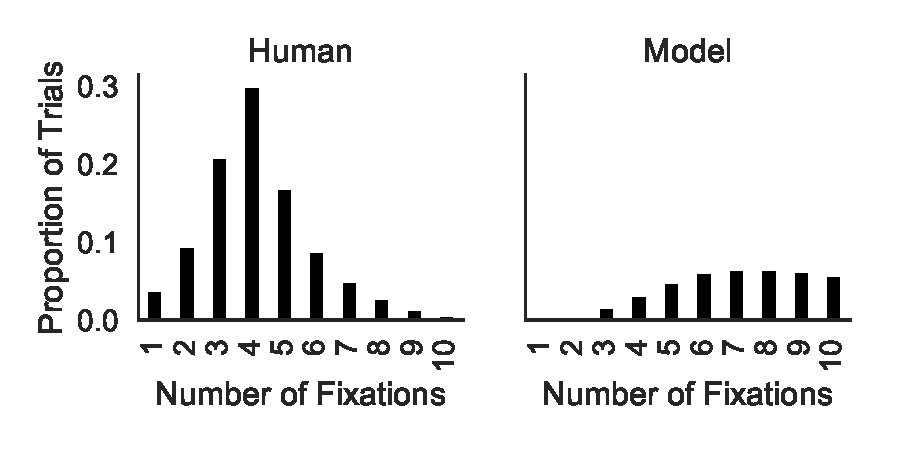
\includegraphics[width=.45\textwidth]{../analysis/figs/nfix.pdf}
      \label{fig:subfig3}
    }
  \caption{Three plots that were used to fit model parameters. (a) shows the relationship between the maximal rating of the shown items and the rating of the chosen item; (b) shows the relationship between how different the ratings are for the candidate items and how long it takes to make a decision; and (b) shows the frequency of different number of fixations, where a model fixation is defined as an unbroken sequence of samples drawn from a single item.}
  \label{fig:loss}
\end{figure}

\subsection{Model fitting}
Although, the parameters of the policy are optimized (reflecting our assumption that people allocate attention rationality), the meta-MDP itself has three free parameters that must be fit to human data.

\begin{enumerate}
  \item $\sigma$ is the standard deviation of the observation distribution that each sample is drawn from. It controls how quickly and reliably the estimates of each item's utility converges to to the true value. Higher values generally result in slower and less accurate decisions.
  \item $\samplecost$ is the cost of taking a sample. It controls how many samples the optimized policy tends to take. Higher values generally result in faster and less accurate decisions.
  \item $\switchcost$ is the additional cost of sampling from a different item than that fixated on the previous time step. Higher values generally result in fewer fixations (changes of attention), and slightly decrease decision time and accuracy.
\end{enumerate}

Ideally, we would optimize these parameters via maximum likelihood estimation. However, there is unfortunately no analytical expression for the likelihood, and it is quite challenging to approximate it by simulation due to the high dimensionality of the data (in particular, the time series of fixations). Thus, we fit the parameters to match three key summary statistics between the model and human data, as shown in Figure~\ref{fig:loss}. In each case, the loss is defined as mean percentage error on each point/bar in the figure. The total loss is simply the sum of these three losses.

To connect the model to behavioral data, we require three additional parameters. The first $\sampletime$ determines how long (in seconds) each sample takes, allowing us to predict fixation and reaction times from the number of samples the model takes. Rather than fitting this parameter, we set it to match the model's mean predicted reaction time (across all trials) to the true mean reaction time. The second and third parameters, $\mu_0$ and $\sigma_0$ allow us to translate the ratings given by participants (on a -10 to +10) scale into values that the model assumes to be unit-normally distributed. The model values are set as $u = \frac{r - \mu_0}{\sigma_0}$. Although these parameters could be fit, we simply validate the model's assumption of unit-normality by setting $\mu_0$ and $\sigma_0$ to the empirical mean and standard deviation of ratings for all items shown in the experiment.

% However, doing so would be equivalent to assuming that people immediately adapt their priors (and as a result, their decision making strategy) to capture the statistics of the experimental task. In particular, because choice trials were restricted to items that were rated positively, we might expect people's priors to be systematically pessimistic, generally being pleasantly surprised by the high values of the items they see. This would correspond to having $\mu_0$ less than the empirical rating mean. If no task-adjustment takes place and people interpret a rating of 0 as average, $\mu_0$ should be set to 0. In practice, we have found (so far) that how we handle these two parameters doesn't matter very much; they seem to trade off with the other parameters somehow so we can get similar quality fits to the human data with any reasonable setting.


\begin{figure}[t!]
  \centering
  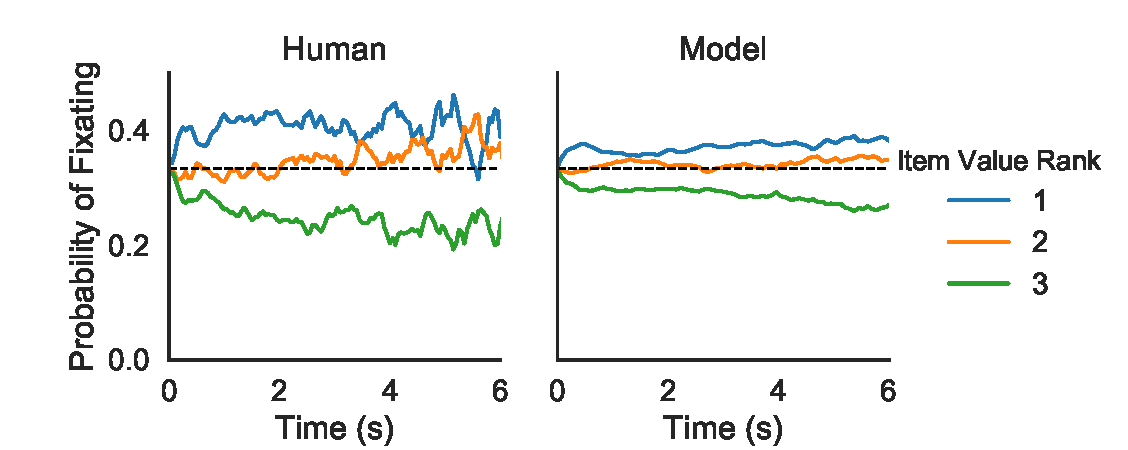
\includegraphics[0.8\textwidth]{../analysis/figs/prob_fix.pdf}
  \caption{The gaze cascade. Over the course of a decision, both humans and the model are increasingly likely to fixate on items with higher rating. Note that the model was not fit to capture this specific effect.}
  \label{fig:attention}
\end{figure}


\section{Results}

The model (comprising the meta-MDP and the optimized policy) makes two key qualitative predictions about the relationships between attention, value, and choice that are relatively insensitive to the specific parameter settings.

\subsubsection{Attention is directed to high-value items}



In our model, the agent is more likely to attend to items that she believes are valuable. To see why this is rational, consider a case in which there are two items with high and similar value and one item with much lower value. The agent can quickly determine that the low value item is not the best one, and thus does not waste any additional time considering it; thus, the two high-value items receive more attention. In the reverse case, in which there is only one high value item, the agent quickly identifies it, and has no reason to determine which of the similarly low valued items is superior; attention is roughly equally divided among the three options. Thus, in net, positively valued items receive more attention.

Importantly, the true value of items does not directly influence attention; this effect is mediated by the internal value estimates that the agent builds over the course of a decision. In the initial stages of a decision, the agent's value estimates will be highly uncertain and noisy, with a weak dependence on the true values. Thus, although she will tend to attend to the item she \emph{believes} is most valuable, it is likely that this item is not truly the most valuable. As the decision progresses, these estimates will become progressively less noisy. Thus, the estimated values that are biasing attention will more closely align with the true values. As a result, we expect to see that the tendency to attend to high value items should increase over the course of the decision. Indeed, as shown in Figure~\ref{fig:attention}, this pattern holds in both the human and simulated model data.

Note that this prediction only holds for decisions between three or more items. Indeed, it has been shown that attention should be exactly evenly divided in the two alternative case \citep{Fudenberg2018}, and our policy optimization method recovers this behavior. Accordingly, no effect of value on attention has been found in two-alternative choice experiments [Antonio: Is this actually true?]

\subsubsection{More attended items are more likely to be chosen}

% \begin{verbatim}
%                   Figure 0

% Mechanism #1: attention -> estimated value -> choice

% Mechanism #2: attention <- estimated value -> choice
% \end{verbatim}


In our model, the more an agent attends to an item, the more likely she is to ultimately choose it. This relationship holds even if we hold the true values constant. Thus, we predict that people will be more likely to choose an item that they looked at more, accounting for any difference in the ratings previously assigned to each item. This prediction is also made by the aDDM, a direct result of the assumption that the drift rate is positively biased towards the attended item. However, our model makes the same prediction without any biases in the evidence accumulation process

There are two mechanisms through which the effect can emerge in our model. The first mechanism is through a mismatch between the prior distribution and the true distribution from which items are drawn. Value estimates in our model are based on a combination of a prior and likelihood, where the weight of the likelihood increases with computation time. Thus, for an item with true value above the prior mean, the estimated value will tend to increase with computation time. Conversely, for an item with value below the prior mean, estimated value will decrease with computation time. This accords with experimental evidence that computation time has opposite effects on the valuation of positive vs. negative items \citep{Armel2008}. If the prior is unbiased, then the positive and negative effects of attention on valuation will wash out. However, if the prior is biased, i.e. if choice items are systematically better or worse than expected, attention will have a corresponding systematic effect on valuation.

The second mechanism by which the apparent attentional bias may emerge depends on the rational allocation of attention. As described in the previous section, the rational model predicts that (in the case of three or more items), the agent will be more likely to attend to an item that she believes is valuable. At the same time, she is also more likely to choose items that she believes are valuable. Thus, a high estimated value makes the agent more likely to both attend to and choose an item. As a result, attention and choice are correlated by a common cause structure. This contrasts to the previous mechanism in which attention has a causal effect on choice, as mediated by estimated value. Importantly, both choice and attention allocation depend on \emph{estimated} value, not the true item values; thus, the correlation is not broken by fixing (conditioning on) true value.

We can distinguish between these two mechanisms by comparing two- vs. three-alternative choice for positive vs. negative items. The biased-prior mechanism is insensitive to the number of alternatives, and will predict a positive (negative) effect of attention when items are generally positive (negative). In contrast, the biased-attention mechanism is insensitive to average value, and will predict a positive effect of attention when there are more than two alternatives, and no effect of attention when there are just two alternatives.

% \setlength{\bibleftmargin}{.125in}
% \setlength{\bibindent}{-\bibleftmargin}
% \renewcommand*{\bibfont}{\footnotesize}
\bibliography{/Users/fred/Dropbox/Miscellaneous/library}


\end{document}